\documentclass[9pt]{beamer}
\usepackage[ngerman,english]{babel}
\usepackage{bibgerm}
\usepackage[autostyle]{csquotes}

\usetheme{TUDOplain}
\setbeamertemplate{navigation symbols}{}
\setbeamertemplate{footline}{\small \vspace{-1ex} \vbox{ \insertframenumber /\inserttotalframenumber}}
\setbeamercovered{invisible}

\author[Merlin Scholz]{Merlin Scholz\\\href{mailto:merlin.scholz@tu-dortmund.de}{merlin.scholz@tu-dortmund.de}}
\title[Analyse der Marsoberfläche durch Unsupervised Learning]{Kategorisieren der Marsoberfläche mithilfe von Unsupervised Learning durch Backpropagation}
\date[20.11.2019]{20. November 2019}
\institute[TU Dortmund]{Mustererkennung,\\ Informatik XII, Technische Universität Dortmund}

\begin{document}
\begin{frame}
	\titlepage
\end{frame}

\begin{frame}{Inhalt}
	\tableofcontents
\end{frame}

\section{Motivation}

\begin{frame}{Motivation: Neuronale Netze zur Bildsegmentierung}
\begin{columns}
	\begin{column}{.5\textwidth}
		\begin{itemize}
			\item Neuronale Netzwerke werden oft zur Bildsegmentierung genutzt
			\item Voraussetzung: Manuell erstellte Ground Truth um das Netzwerk zu trainieren
			\end{itemize}
	\end{column}
	\begin{column}{.5\textwidth}
		\begin{figure}[H]
			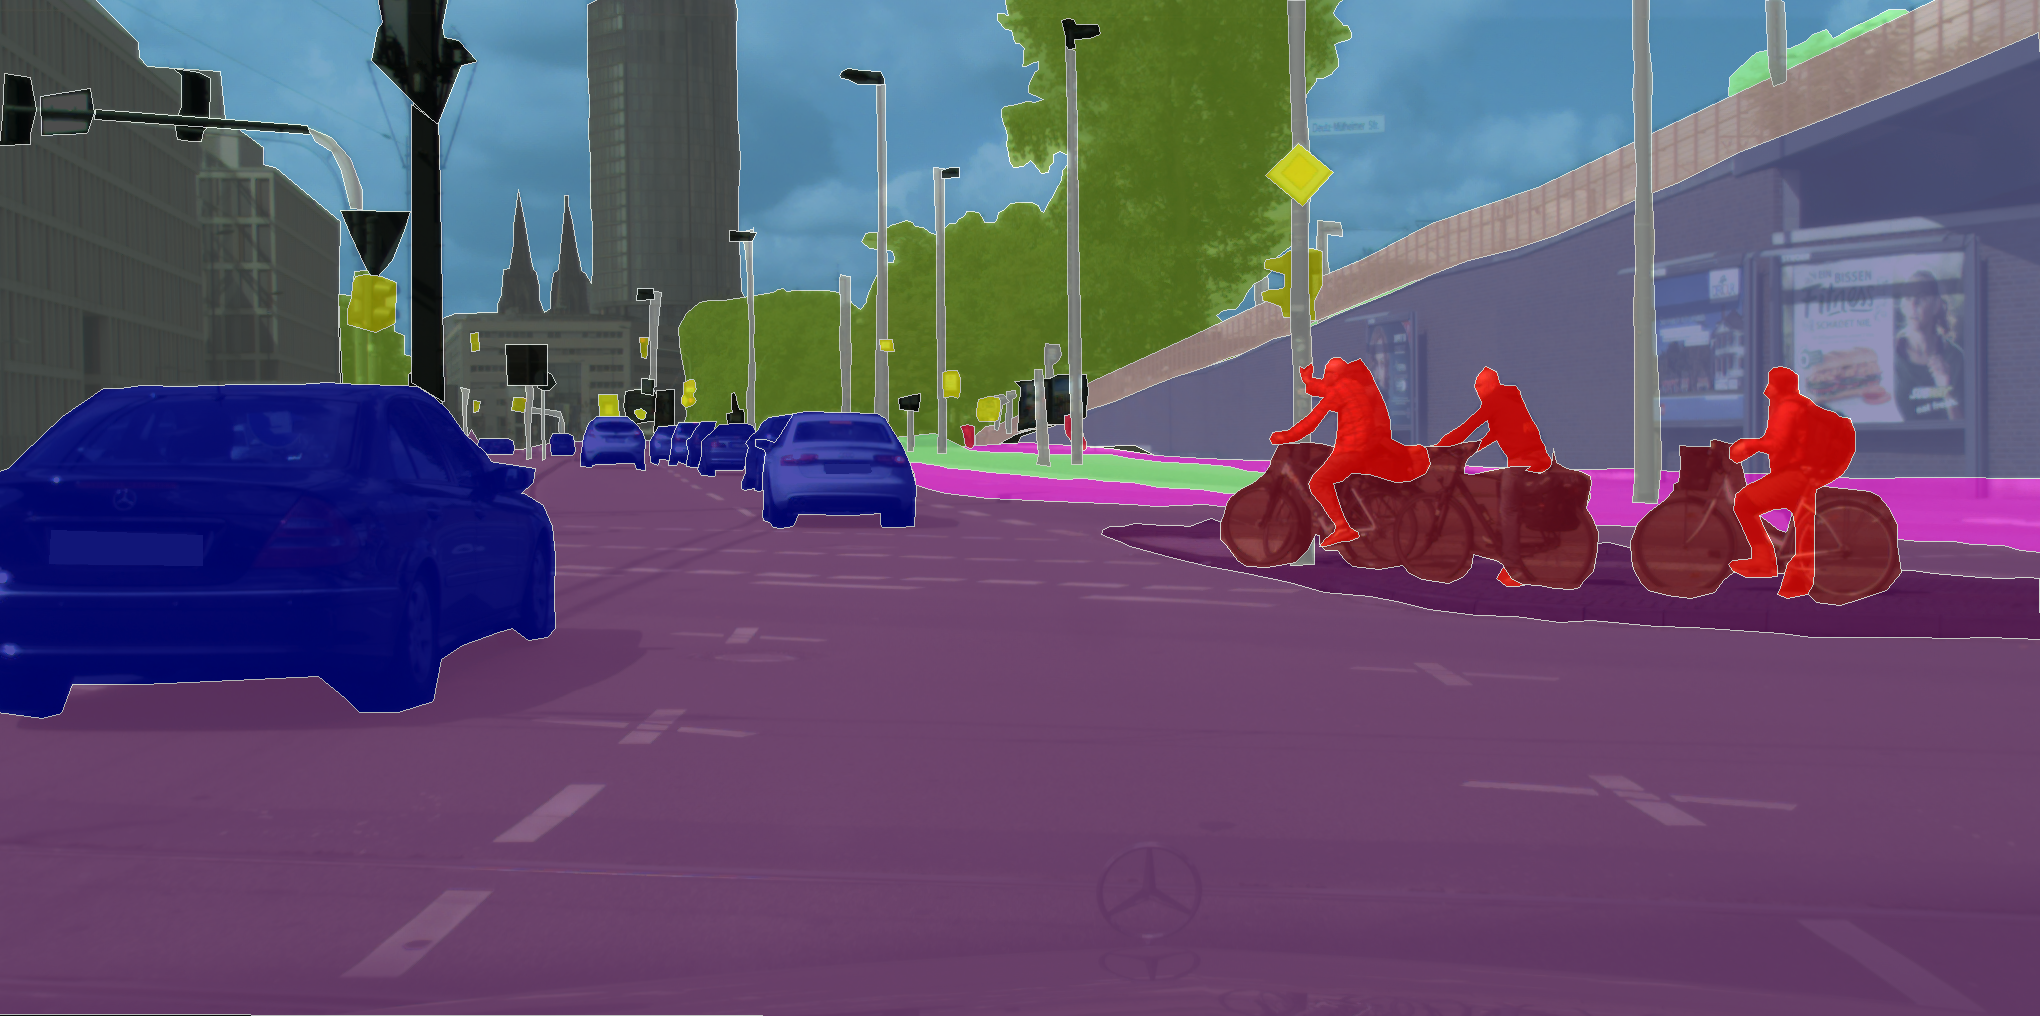
\includegraphics[width=\textwidth,keepaspectratio]{koeln00.png}
			\caption{Beispiel: CityScapes Dataset\cite{Cordts_2016_CVPR}}
		\end{figure}
	\end{column}
\end{columns}
\end{frame}

\begin{frame}{Motivation: (Fehlende) Ground Truths}
Ground Truth nicht immer vorhanden: Beispiel Marsoberfläche
\begin{itemize}
	\item Zu großer Datensatz
	\item Notwendigkeit von Experten
	\item[$\Rightarrow$] Manuelle Erstellung nicht kostengünstig oder zeiteffizient möglich
\end{itemize}
\medskip
Lösungsansatz:
\begin{itemize}
	\item Anfangs zufällige Klassifizierung durch Segmentierungsalgorithmus weiter optimieren
\end{itemize}
\end{frame}

\section{Verwandte Arbeiten}

\begin{frame}{Verwandte Arbeiten: Segmentierung nach Kanezaki\cite{kanezaki2018_unsupervised_segmentation}}
\begin{columns}
	\begin{column}{.5\textwidth}
		\begin{itemize}
			\item Unüberwachtes Lernen der Segmentierung
			\item Anfangs zufällige Ergebnisse werden mit Clusteringalgorithmus vereint
			\item Zielfunktion: Softmax-Loss zwischen Ergebnis des NN und des optimierten Ergebnisses
			\item NN wird auf diese Zielfunktion hin optimiert (Backpropagation)
		\end{itemize}
	\end{column}
	\begin{column}{.5\textwidth}
		\begin{figure}
			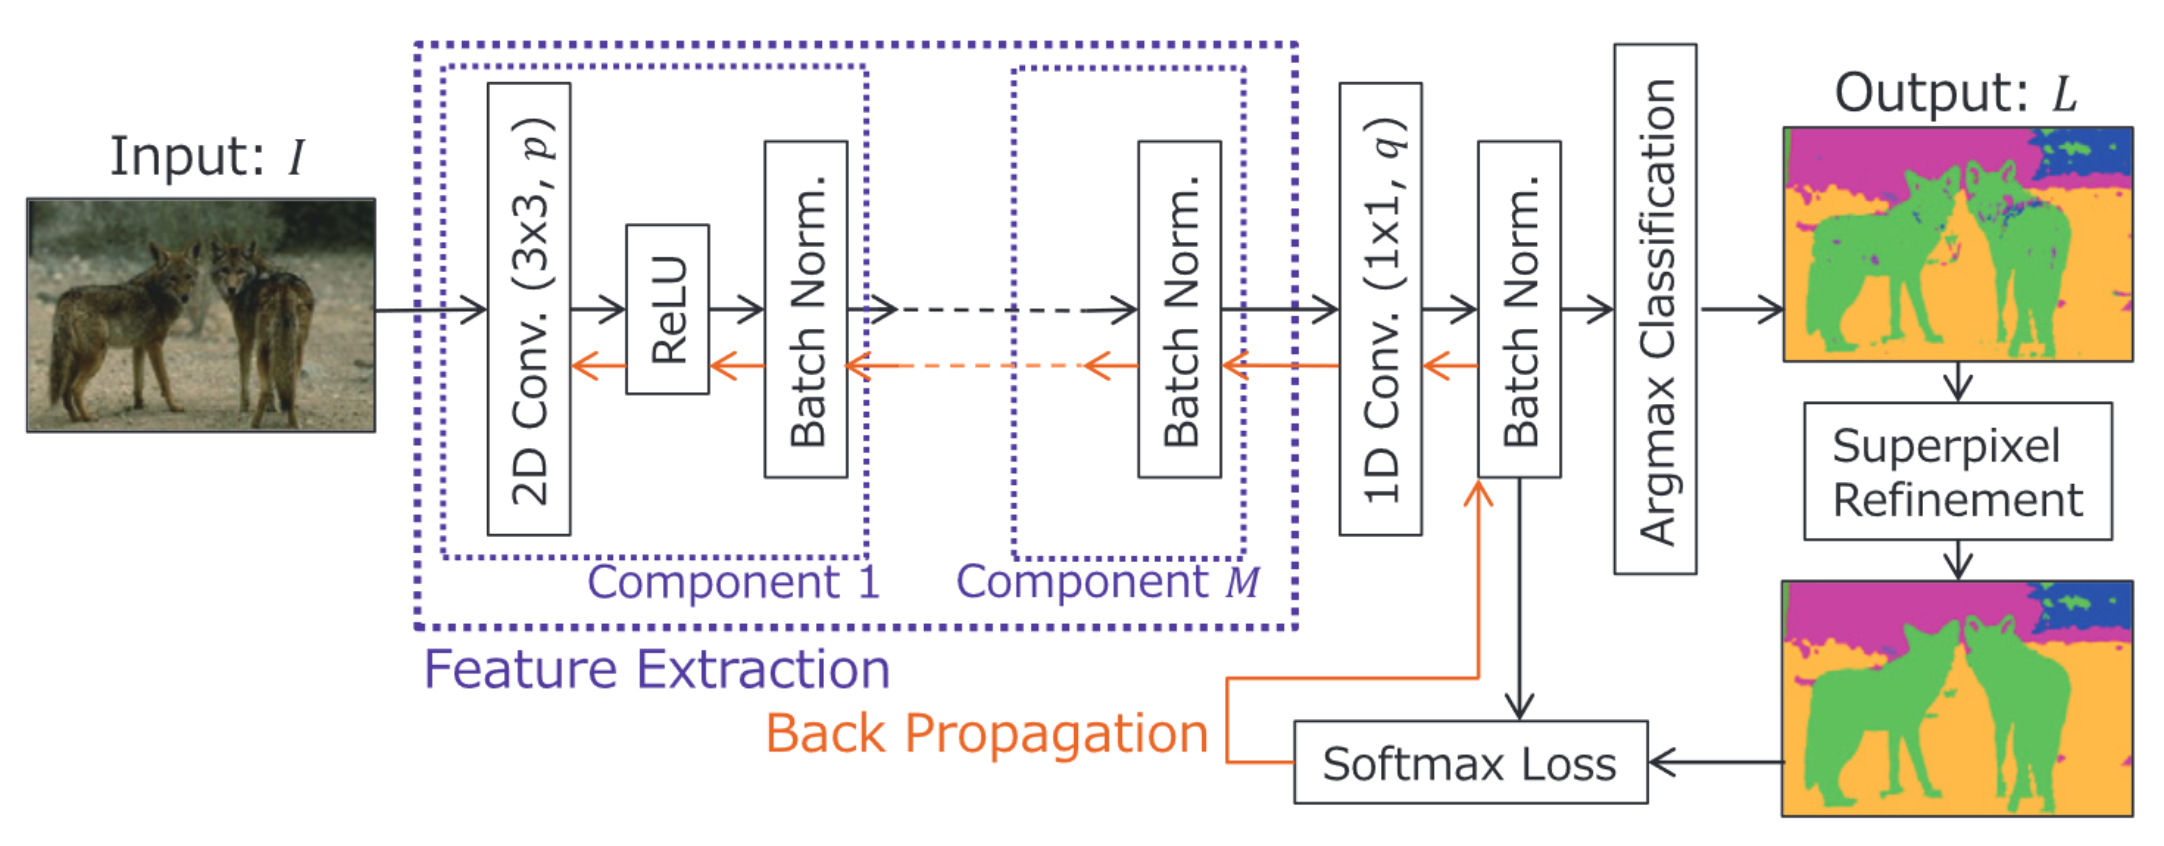
\includegraphics[width=\textwidth,keepaspectratio]{kanezaki.png}
			\caption{Vorgehensweise nach Kanezaki\cite{kanezaki2018_unsupervised_segmentation}}
		\end{figure}
	\end{column}
\end{columns}
\end{frame}

\begin{frame}{Detection of craters [...] using shape and texture features nach Bandeira\cite{Bandeira2012}}
\begin{columns}
	\begin{column}{.5\textwidth}
		\begin{enumerate}
		\item Vorsortierung basierend auf Urbach \& Stepinskis Algorithmus\cite{urbach2009automatic} zur Kratererkennung
		\begin{itemize}
			\item Effiziente Methode zur Krater-Erkennung
			\item 70\% Erkennungsrate
			\item Funktionsweise über Schatten und Highlights
		\end{itemize}
		\item Überlagerung von 9 Bitmasken (in versch. Positionen) und Prüfung auf Übereinstimmungen
		\item Anwendung eines angepassten AdaBoost Algorithmus
		\item Post-Processing: Eliminierung von ungewöhnlich geformten Kratern
		\end{enumerate}
	\end{column}
	\begin{column}{.5\textwidth}
		\begin{figure}[H]
			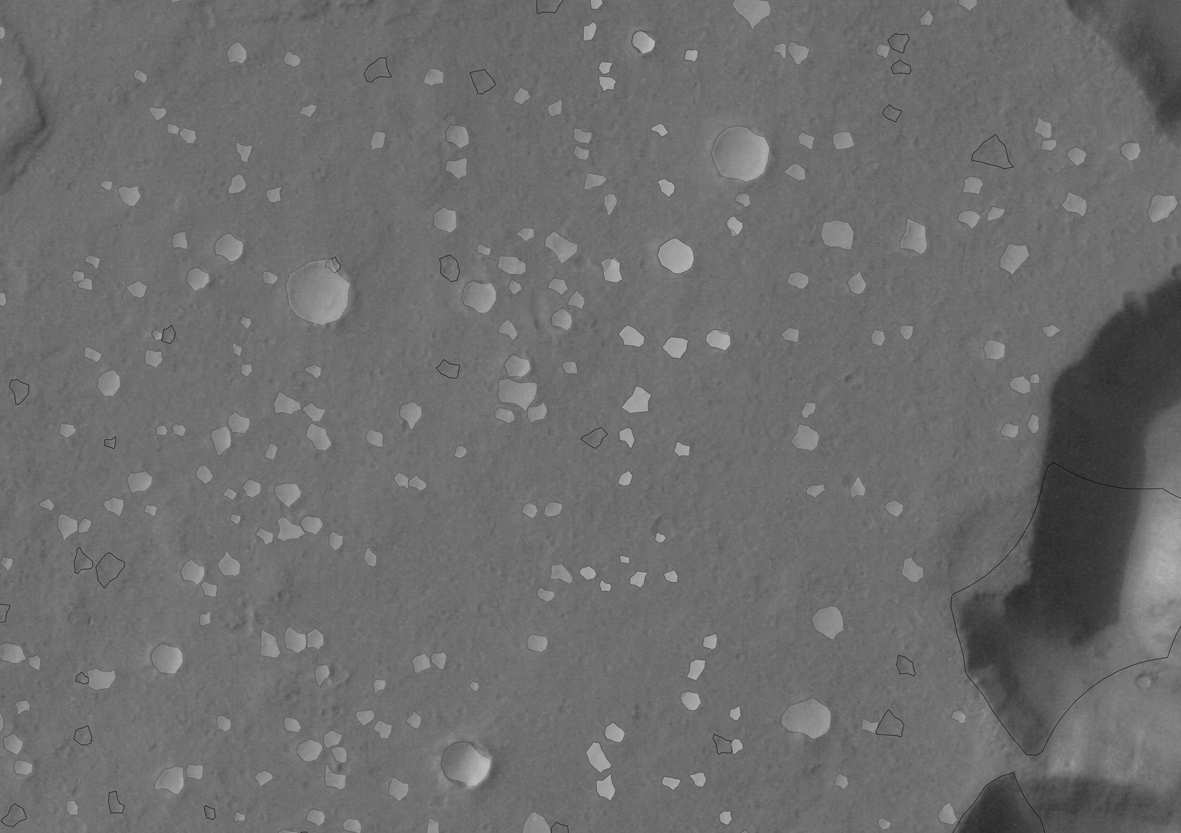
\includegraphics[width=\textwidth, keepaspectratio]{bandeira_detected.png}
			\caption{Erkannte Krater nach Bandeira\cite{Bandeira2012}}
		\end{figure}
	\end{column}
\end{columns}
\bigskip
\begin{center}Hierauf basierend: Der Krater-Datensatz der University of Massachusetts\cite{umass_craters} (vergleichbar mit unserem Ziel)
\end{center}
\end{frame}

\begin{frame}{Verwandte Arbeiten: \textit{Crater Detection via CNNs}\cite{2016arXiv160100978C}}
\begin{itemize}
	\item Erforscht Neuronale Netze statt manuell erstellten Gabor-/ Sobel-Filtern
	\item \enquote{Klassischer} Ansatz über neuronale Netze
	\item Lernt auf Bandeira-Datensatz der UMass\cite{umass_craters}
	\item Nutzt F1-Score und Cross Validation zur Evaluierung
	\item Gute Ergebnisse, F1-Score zwischen $88\%$ und $91\%$ (vgl. Bandeira $79\%-86\%$)
\end{itemize}
\end{frame}

\section{Vorgehensweise}

\begin{frame}{Vorgehensweise: Datensatz}
		
\end{frame}

\begin{frame}{Vorgehensweise: Implementierung}
\begin{itemize}
	\item Grundlegende Idee ähnlich zu Kanezaki\cite{kanezaki2018_unsupervised_segmentation}, basierend auf PyTorch
	\item Benutzung von Python Bibliotheken nicht immer möglich (zu große Eingabedaten, bspw. bei SLIC\cite{slic})
	\item[$\Rightarrow$] Speichereffizienter neu implementieren, ggf. über Sliding-Window-Verfahren
	\item Für bessere Performance wird oft auf Cython\cite{behnel2010cython} zurück gegriffen
\end{itemize}	
\end{frame}

\begin{frame}{Vorgehensweise: Erweiterung}
Zur Optimierung der Ergebnisse werden einzelne Teile des Algorithmus ersetzt:
\begin{itemize}
	\item Ersetzen des relativ einfachen Neuronalen Netzes durch größere, bspw. ImageNet, Faster R-CNNs, YOLOv3, etc.
	\item Ersetzen des SLIC Clusteringalgorithmus durch bspw. k-Means Clustering oder Mean-Shift Clustering
\end{itemize}	
\end{frame}

\begin{frame}{Vorgehensweise: Evaluierung (1)}
Um die Alternativen evaluieren zu können, wird der Algorithmus auf Datensätze mit vorhandenen Ground Truths angewandt:
\medskip
\begin{itemize}
	\item \textit{Common Objects In Context}\cite{LMBHPRDZ:ECCV:2014} oder das \textit{Cityscapes Dataset}\cite{Cordts2016Cityscapes}
	\item[$\Rightarrow$] Weit verbreitete Datensätze zur Bildsegmentierung
	\medskip
	\item \textit{The Prague Texture Segmentation Datagenerator and Benchmark}\cite{mikevs2015benchmarking}
	\item[$\Rightarrow$] Den zu analysierenden Daten sehr ähnlich, also realitätsnaher
\end{itemize}
\end{frame}

\begin{frame}{Vorgehensweise: Evaluierung (2)}
Die generierten Resultate werden mit den jeweils zugehörigen Ground Truths verglichen, bspw. über F1-Score
\pause
\begin{block}{Hinweis}
	Metriken, die auf Clusterlabels basieren sind nur eingeschränkt nutzbar
\end{block}
\pause
\begin{block}{Hinweis}
	Zum Vergleich müssen die jeweiligen NNs den selben Seed nutzen
\end{block}
\end{frame}

\begin{frame}{Vorgehensweise: Optimierungen}
	\begin{itemize}
		\item Eingabebilder in Graustufen: Optimierung des Clusterings und des NNs
		\item Parallelisierung entweder pro Bild oder mehrere Bilder parallel
		\item Wahl des am besten geeigneten Clustering-Algorithmus
		\item Wahl des am besten geeigneten Aufbaus des NNs
	\end{itemize}
\end{frame}

\section{Referenzen}

\begin{frame}[shrink=25]{Referenzen}
	\bibliographystyle{gerabbrv3}
	\bibliography{presentation}
\end{frame}

	
\end{document}